\let\negmedspace\undefined
\let\negthickspace\undefined
\documentclass[journal]{IEEEtran}
\usepackage[a5paper, margin=10mm, onecolumn]{geometry}
%\usepackage{lmodern} % Ensure lmodern is loaded for pdflatex
\usepackage{tfrupee} % Include tfrupee package

\setlength{\headheight}{1cm} % Set the height of the header box
\setlength{\headsep}{0mm}     % Set the distance between the header box and the top of the text

\usepackage{gvv-book}
\usepackage{gvv}
\usepackage{cite}
\usepackage{amsmath,amssymb,amsfonts,amsthm}
\usepackage{algorithmic}
\usepackage{graphicx}
\usepackage{textcomp}
\usepackage{xcolor}
\usepackage{txfonts}
\usepackage{listings}
\usepackage{enumitem}
\usepackage{mathtools}
\usepackage{gensymb}
\usepackage{comment}
\usepackage[breaklinks=true]{hyperref}
\usepackage{tkz-euclide} 
\usepackage{listings}
% \usepackage{gvv}                               

\def\inputGnumericTable{}                      
\usepackage[latin1]{inputenc}                    
\usepackage{color}                              
\usepackage{array}                             
\usepackage{longtable}                          
\usepackage{calc}                               
\usepackage{multirow}                           
\usepackage{hhline}                            
\usepackage{ifthen}                          
\usepackage{lscape}
\begin{document}

\bibliographystyle{IEEEtran}
\vspace{3cm}

\title{1.7.9}
\author{AI25BTECH11023 - Pratik R
}
% \maketitle
% \newpage
% \bigskip
{\let\newpage\relax\maketitle}

\renewcommand{\thefigure}{\theenumi}
\renewcommand{\thetable}{\theenumi}
\setlength{\intextsep}{10pt} % Space between text and floats


\numberwithin{equation}{enumi}
\numberwithin{figure}{enumi}
\renewcommand{\thetable}{\theenumi}


\textbf{Question: }\\
If the points $\vec A= (k + 1,2k)$, $\vec B= (3k,2k + 3)$, and $\vec C= (5k-1,5k)$ are collinear, then
find the value of k.

\textbf{Solution: } \\
Given that
$$
\vec A = \myvec {k+1 \\ 2k}, \vec B = \myvec{3k \\ 2k+3}, \vec C = \myvec{5k-1 \\ 5k}.
$$
$\vec A$, $\vec B$ and $\vec C$ are collinear therefore

\begin{align}
    rank \brak{\vec B- \vec A, \vec C -\vec A}=1 
\end{align}
\begin{align}
    (\vec B-\vec A) = \myvec{2k-1 \\ 3}\\ (\vec C-\vec A) = \myvec{4k-2 \\ 3k}
\end{align}
 \begin{align}
     \myvec {\vec B -\vec A && \vec C -\vec A}^T =\myvec{2k-1 && 3 \\ 4k-2&& 3k}  
 \end{align}
$R_2 \to R_2 - (R_1\times 2):$
 \begin{align}
 = \myvec{2k-1 && 3 \\ 0 && 3k-6}
 \end{align}
For rank = 1,
\begin{align}
    3k -6 = 0 \implies k = 2
\end{align}
Hence , the value of k is 2.

\begin{figure}[h!]
    \centering
    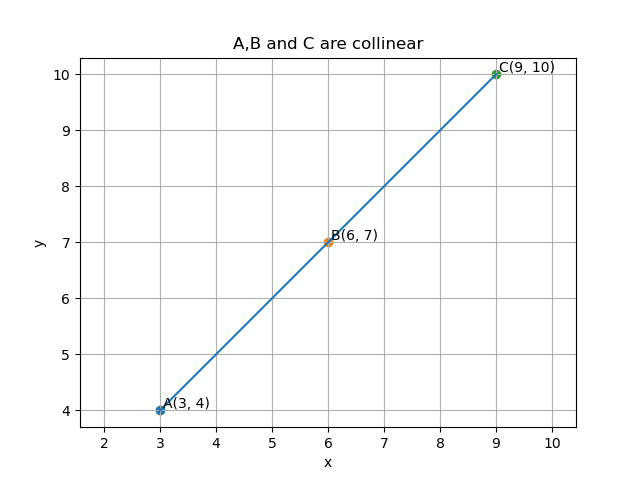
\includegraphics[width=0.7\columnwidth]{figs/fig.png}
    \caption{}
\end{figure}


\end{document}